\section{Use case diagram}
\subsection{Introduction}
\begin{flushleft}
La plus grande différence réside dans \textbf{les accès aux portefeuilles}.
\end{flushleft}

\begin{flushleft}
Pour cette raison, j’ai choisi de \textbf{séparer} la partie « Voir les portefeuilles » où il s’agit de portefeuilles appartenant entièrement au client \textbf{« gestionnaire »}, de la partie « voir les portefeuilles où il est invité » pour permettre une meilleure visibilité des cas.
\end{flushleft}

\subsection{Client}
\begin{flushleft}
Lorsque le client ou plus précisément, le gestionnaire du portefeuille est sur la section « Voir les portefeuilles », il pourra créer ou fermer un portefeuille et voir les données de consommation du portefeuille comme sur la base du projet.
\end{flushleft} 

\begin{flushleft}
Ce dernier sera également apte à gérer ces données et à voir les utilisateurs invités sur ses portefeuilles étant donné son « grade » de gestionnaire. 
\end{flushleft}

\begin{flushleft}
A partir de cette option, le gestionnaire aura la capacité d’ajouter, supprimer des utilisateurs ou gérer les permissions de ces derniers.
\end{flushleft}

\begin{flushleft}
Une fois sur la section « Voir les portefeuilles où il est invité », le client aura accès à la visualisation des données en lecture seule et à cette même option ainsi qu’à gérer les données en lecture et écriture. 
S’il n’a pas les permissions requises pour gérer les données, l’accès sera \textbf{refusé}.
\end{flushleft}

\begin{flushleft}
Celui-ci aura aussi la possibilité de quitter un portefeuille lorsqu’il le souhaite.
\end{flushleft}

\newpage

\begin{figure}[h]
\subsection{Diagramme}
\centering
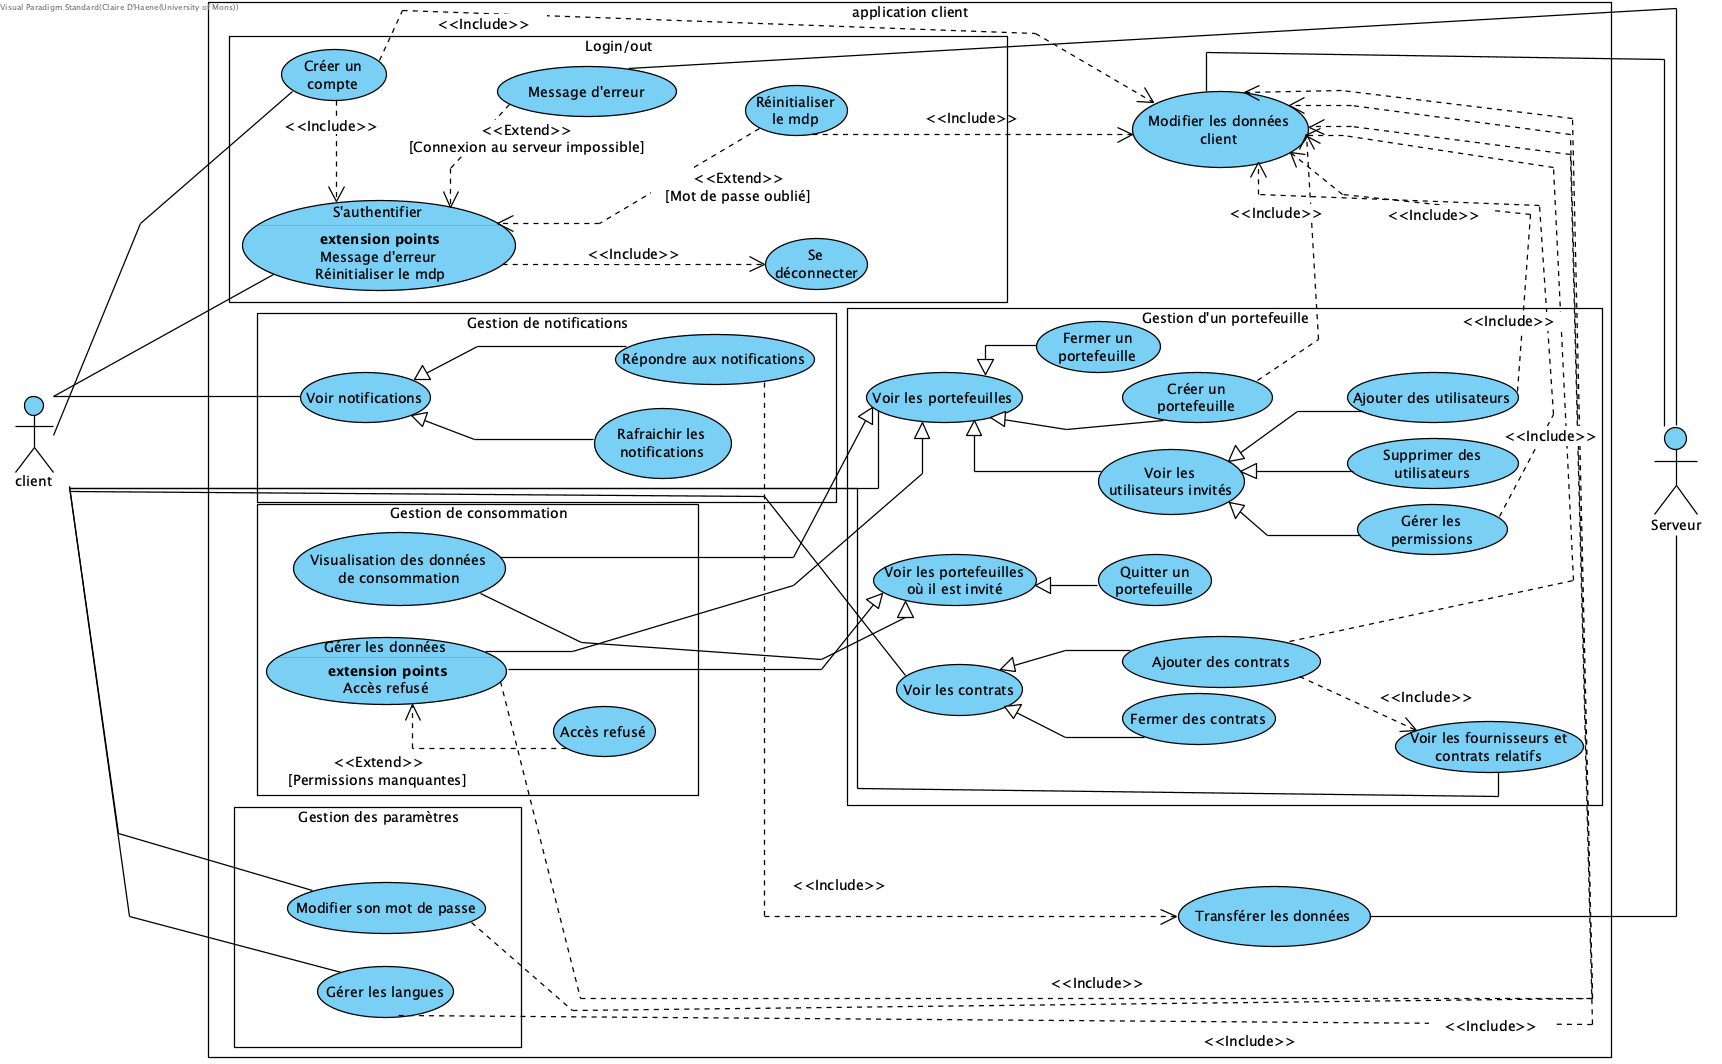
\includegraphics[width = 1\textwidth]{Extension-claire/Usecase-claire/img/usecase.png}
\end{figure}
